\documentclass[a4paper, 11pt]{article}

\usepackage{amsmath}
\usepackage{amssymb}
\usepackage{hyperref}
\usepackage{makeidx}
\usepackage{graphicx}
\graphicspath{{figures/}} % Directory in which figures are stored
\usepackage{natbib}% \bibliography
\usepackage{float}
\usepackage{setspace} % for line spacing
\usepackage[margin=1in]{geometry}
\usepackage[skip=2pt]{caption} 
\title{Assignment2-CSE780}
\author{Paria, Fakhrzad \\ Stuent ID: 400353290 }
\date{7-October-2021}
\setstretch{1.5}

\begin{document}
	
	\maketitle
	\newpage
\section*{a.Describe the data}
we will use a Car insurance claim dataset in 2021 that has collected based on customers of that insurance company ~\cite{data}. there are 10000 customer as sample in this data frame. Also 17 features have been collected based on the customer's attributes. There is one column that shows this customer had accident claim last year or not. this is logical column. The data shows that 23percent of customers claimed the accident insurance last year.
	
\section*{b.Exploratory data analysis}	
\subsection*{b.1 Summary and Data Cleanup}
Following table1 is summary of customer attributes. The rows with NA values in SpeedingViolation have been removed. Also the age and experience were interval that both have converted to Number(by mean of interval). Other char columns(gender, married,education,...), now are factors with this logic:
Gender female=1 , male=0 - married True=1 , false=0 - 
children True=1 , false=0
\begin{table}[H]
	\centering
	\caption{Customer dataset attributes}
	\label{table1}
	\begin{tabular}{clllllll}
		\hline
		&  \textbf{age} & 	\textbf{gender} & driving\_experience & married & children &  postal\_code  \\ 
		\hline
		type &num   &Factor  & num &Factor  & Factor&num \\ 
		X & Min. :20 & 0:9043 & Min. : 5 & 0:9043 & 0:9043  & Min.:10238  \\ 
		X.1 & Median :33   &  & Median :15   &  &  & Median :10238    \\ 
		X.2 & Mean   :42.38   &  & Mean   :15.76   &  &  & Mean   :19788    \\ 
		X.3 & Max.   :65   &  & Max.   :35   &  &  & Max.   :92101    \\ 
		\hline
	\end{tabular}
\end{table}

\begin{table}[H]
	\centering
	\begin{tabular}{clllll}
		\hline
		&     race &  education &           income &  credit\_score & vehicle\_year \\ 
		\hline
		type &Factor   &Factor   & Factor  &num    & Factor  \\ 
		X & Length:9043        & 0:9043        & 0:9043   & Min.   :0.0534   & 0:9043        \\ 
		X.1 &    &    & upper class  :3946   & Median :0.5268   &    \\ 
		X.2 &  &  & working class:1546   & Mean   :0.5164   &  \\ 
		X.3 &  &  &  & Max.   :0.9608   &  \\ 
		\hline
	\end{tabular}
\end{table}

\begin{table}[H]
	\centering
	\begin{tabular}{clllll}
		\hline
		& vehicle\_ownership & vehicle\_type & annual\_mileage & speeding\_violations & past\_accidents \\ 
		\hline
		type &Factor    & Factor    & num         &num       & num \\
		X    & 0:9043   & 0:9043    & Min. : 2000 & Min. : 0 & Min.: 0 \\ 
		X.2 &  &  & Median :12000   & Median : 0 & Median : 0   \\ 
		X.3 &  &  & Mean   :11697   & Mean   : 1.491 & Mean   : 1.066 \\ 
		X.5 &  &  & Max.   :22000   & Max.   :22.000 & Max.   :15  \\ 
		X.6 &  &  & NA's  :957      &                &  \\
		\hline
	\end{tabular}
\end{table}


\subsection*{b.2 pairwise correlation}
In this section we tried to explore the association by visualization tools and some statistical evidence.
In first step we used xtabs() to verify that all levels of factor variables had both claimed insurance.
Then we use ggpairs() \cite{Emersonetc2012} to see correlation between numeric features in figure1. the significant point is that Age and driving experience are collinear.  In figure4 It appears that older  customers who own the vehicle tended to not claim the insurance for accident(outcome in figure legend) than those who did not. Also in figure5 it seems there are relationship between credit score and number of claims in last year.

\begin{figure}[H]
	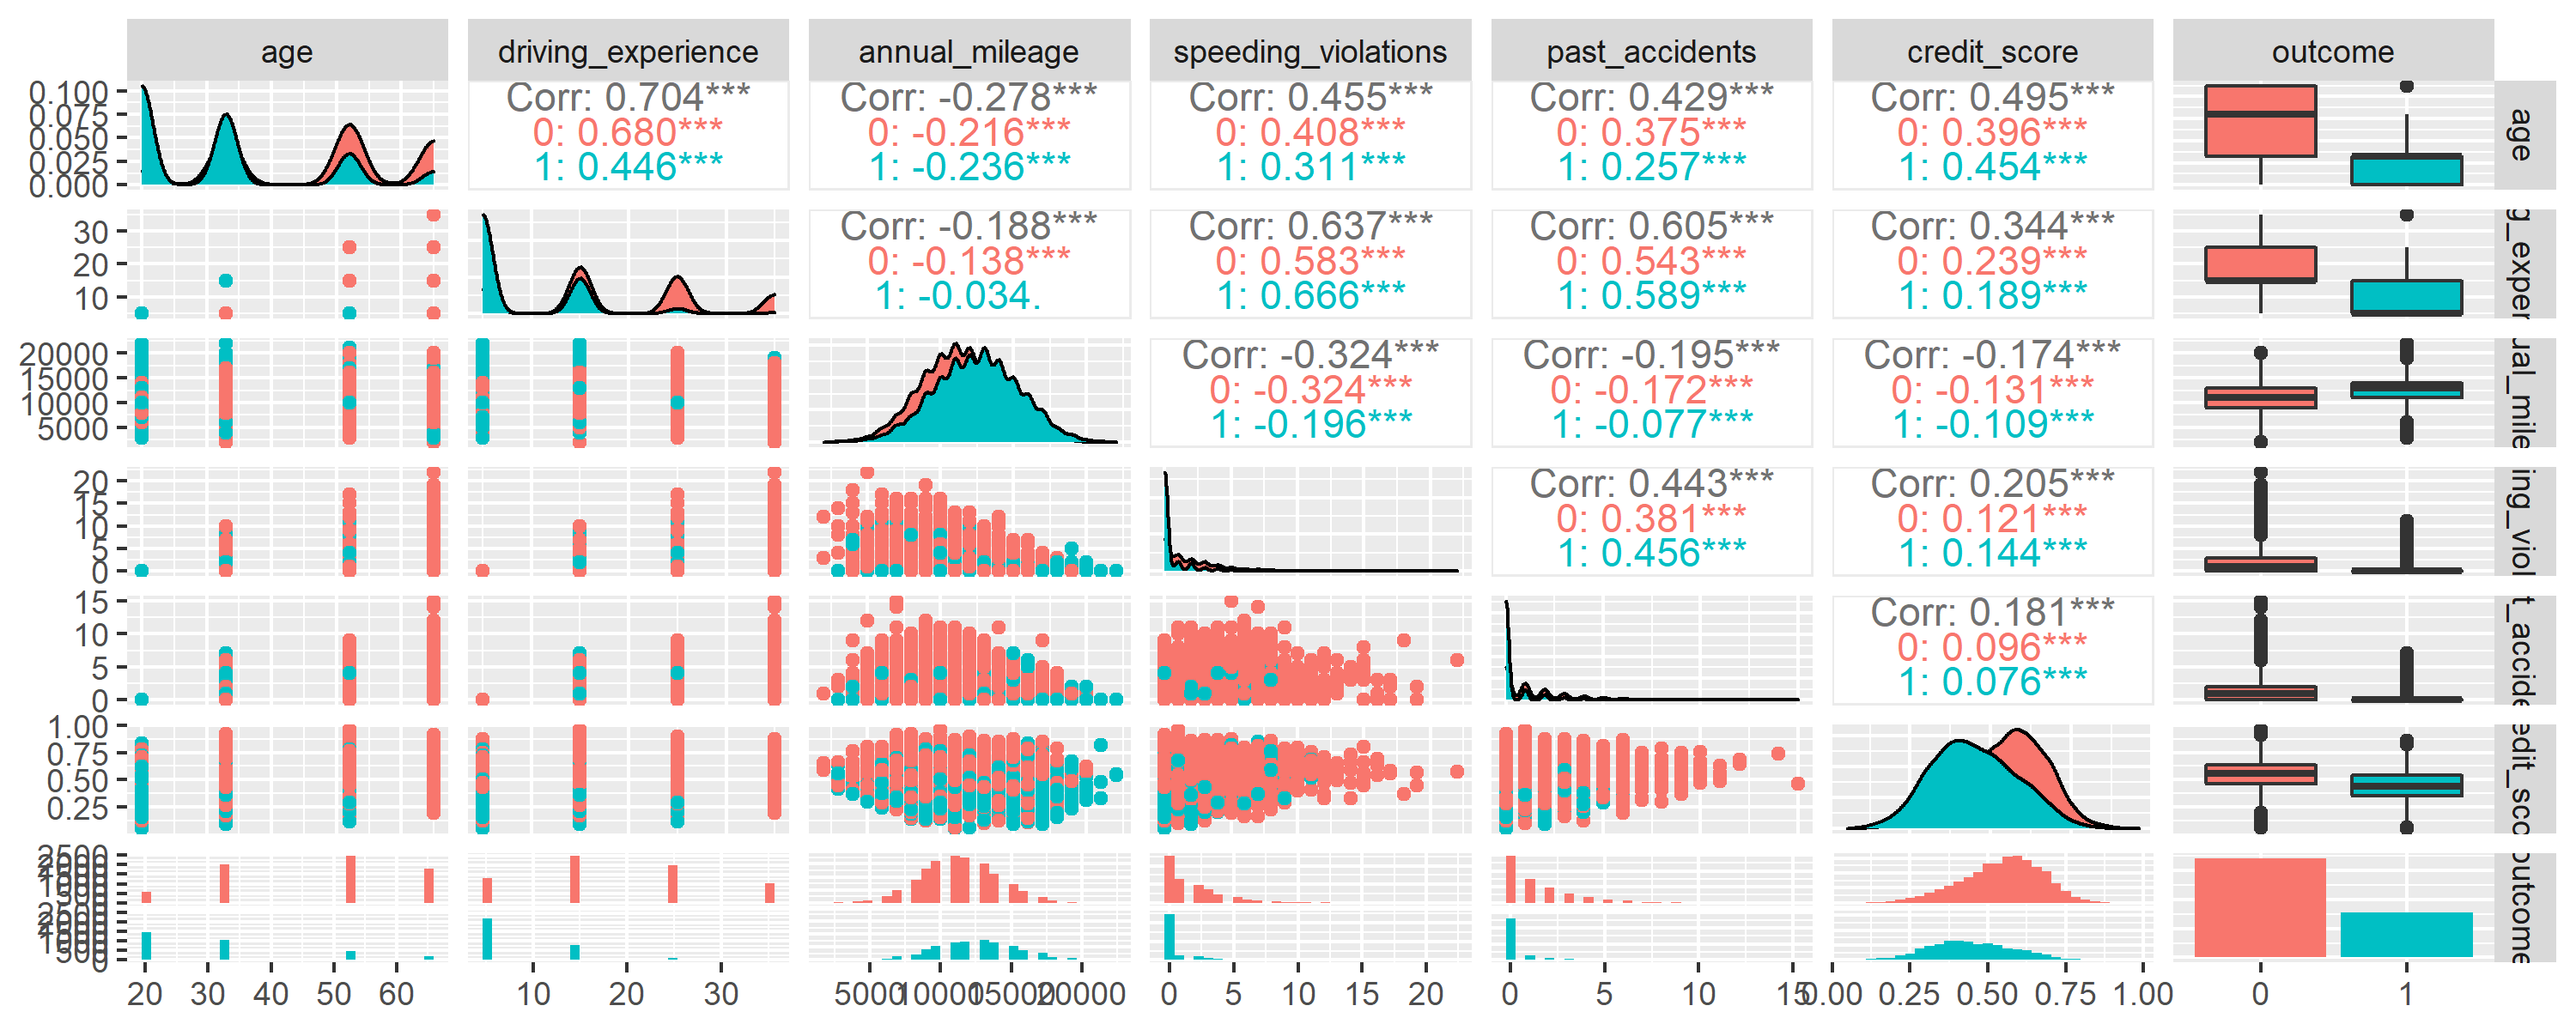
\includegraphics[width = \textwidth]{figure1.png}
	\caption{Pairwise Correlation}
	\label{Figure1}
\end{figure}


\begin{figure}[H]
	\centering
	\begin{minipage}[b]{0.4\textwidth}
		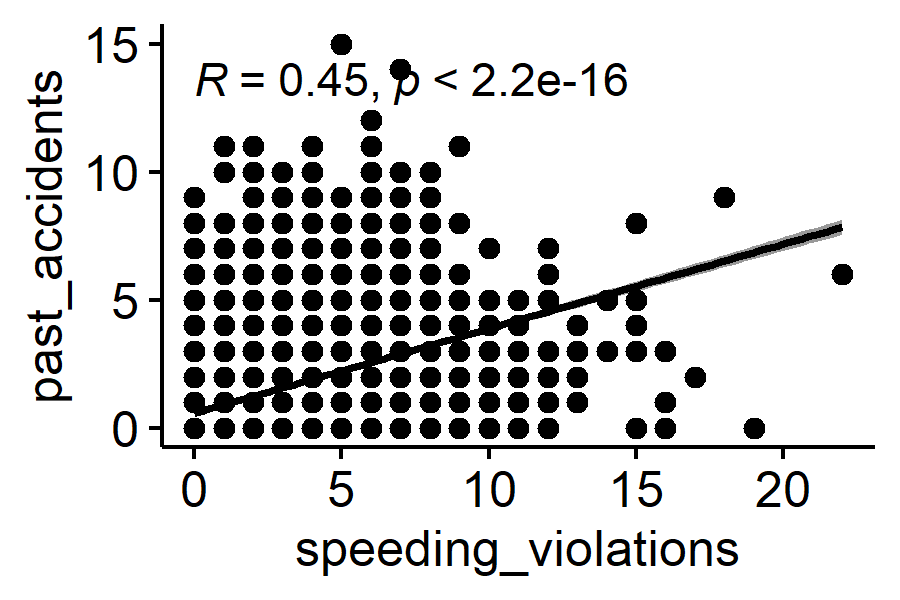
\includegraphics[width=\textwidth]{figure2.png}
		\caption{}
	\end{minipage}
	\begin{minipage}[b]{0.4\textwidth}
		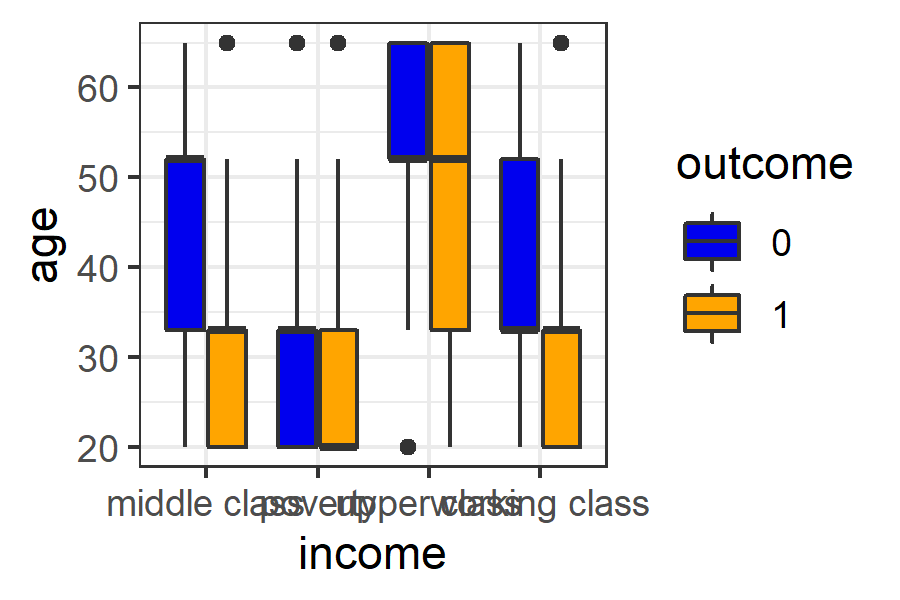
\includegraphics[width=\textwidth]{figure3.png}
		\caption{}
	\end{minipage}
	\hfill
	\begin{minipage}[b]{0.4\textwidth}
	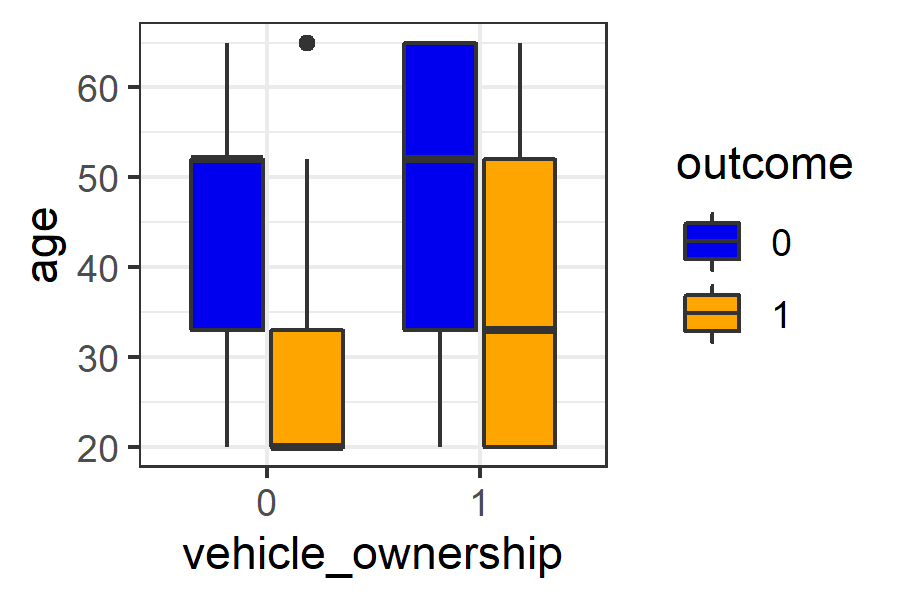
\includegraphics[width=\textwidth]{figure4.png}
	\caption{}
     \end{minipage}
 	\begin{minipage}[b]{0.4\textwidth}
 	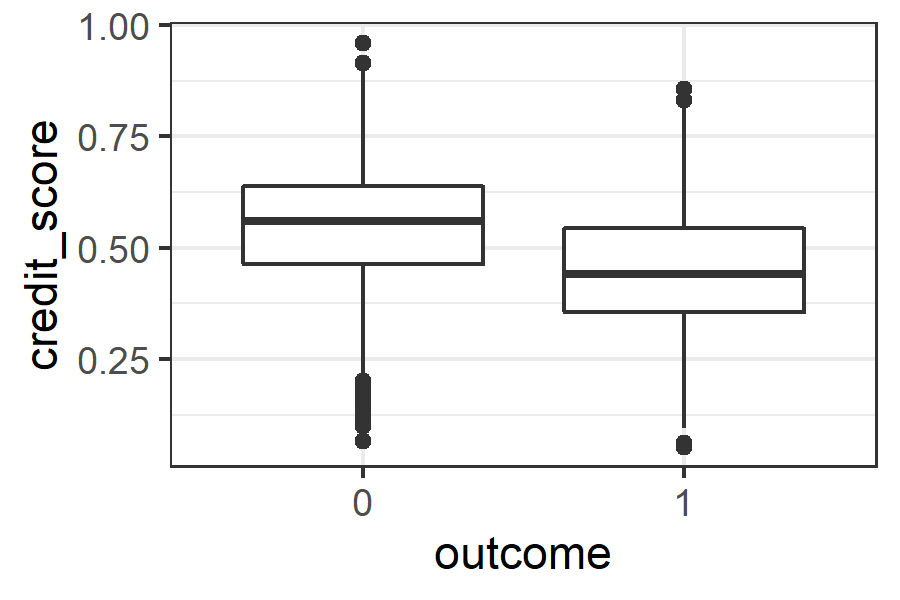
\includegraphics[width=\textwidth]{figure5.png}
 	\caption{outcome is insurance claim}
 \end{minipage}
\end{figure}


\section*{c.Classification}	
The data has splitted randomly to 0.75 as training and 0.25 as testing. and we fit the models with training data then we predict the response with test data. we used two KNN and logistic regression models. we used backward way for feature selection in our model and check our model's accuracy to see the result.

\subsection*{c.1  K-nearest neighbour}
For this classification model we need K that based on this link generally one of the ways for calculating is sqrt(n) that n is sample size. Also we can run our model with different list of K and choose the best result that you can see the result in table.
\begin{table}[H]
	\centering
	\caption{K determination}
	\label{table2}
	\begin{tabular}{rr}
		\hline
		 K & Accuracy \\ 
		\hline
		43 & 0.7938  \\ 
		33 & 0.7934  \\ 
		31 & 0.7930  \\ 
		27 & 0.7925 \\ 
		45 & 0.7921 \\ 
		29 & 0.7916  \\ 
		\hline
	\end{tabular}
\end{table}
We fit the model with K=43 and train and test samples. we repeat the model 10 times for recording the accuracy as table3.
 \begin{table}[H]
 	\centering
 	\caption{Prediction Accuracy }
 	\label{table3}
 	\begin{tabular}{cc}
 		\hline
 		 Run & KNN Accuracy \\ 
 		\hline
 		1 & 0.79 \\ 
 		2 & 0.78 \\ 
 		3 & 0.75 \\ 
 		4 & 0.79 \\ 
 		5 & 0.78 \\ 
 		6 & 0.77 \\ 
 		7 & 0.79 \\ 
 		8 & 0.78 \\ 
 		9 & 0.78 \\ 
 		10 & 0.77\\ 
 		Ave & 0.7830\\
 		\hline
 	\end{tabular}
 		\quad
 \begin{tabular}{c}
 	\hline
 	LR Accuracy \\ 
 	\hline
 	0.80 \\ 
 	0.81  \\ 
 	 0.83  \\ 
 	 0.83  \\ 
 	 0.82  \\ 
 	 0.82  \\ 
 	 0.82  \\ 
 	 0.81  \\ 
 	 0.81  \\ 
 	 0.80  \\ 
    0.8139 \\
 	\hline
 \end{tabular}		
 \end{table}

\subsection*{c.2 logistic regression }
We fit model logistic regression based on the train and test data and run it 10 times. Also we consider that labels with fitted probability more than 50\% are correct and we plot the accuracy probability with samples as figure6. It clearly shows that the logistic regression model works well based on this dataset. Also based on figure8 it shows there is not much outlier. 

\begin{figure}[H]
	\begin{minipage}{0.5\textwidth}
	\centering
	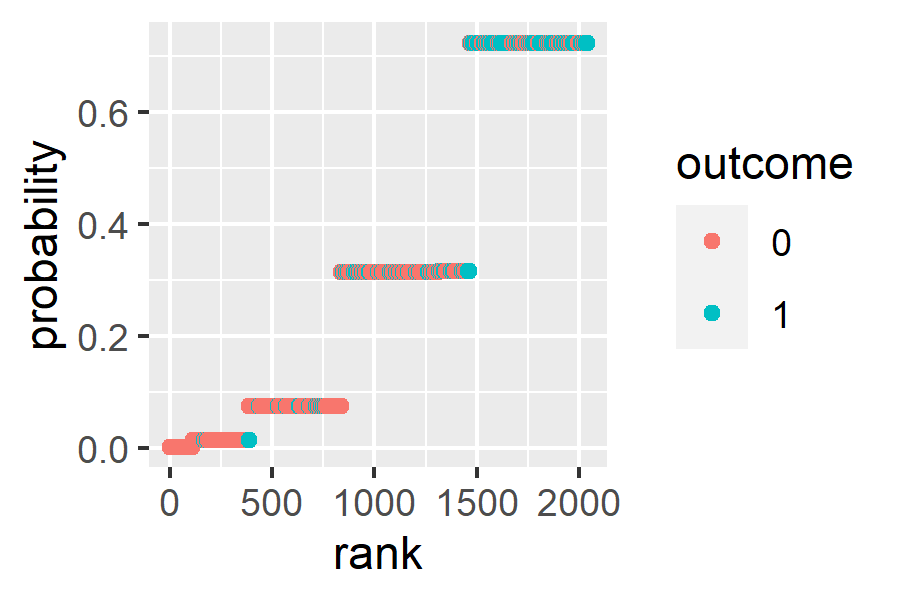
\includegraphics[width = \textwidth]{figure7.png}
	\caption{logistic regression fitted probability}
	\label{Figure6}
	\end{minipage}
	\begin{minipage}{0.5\textwidth}
	\centering
	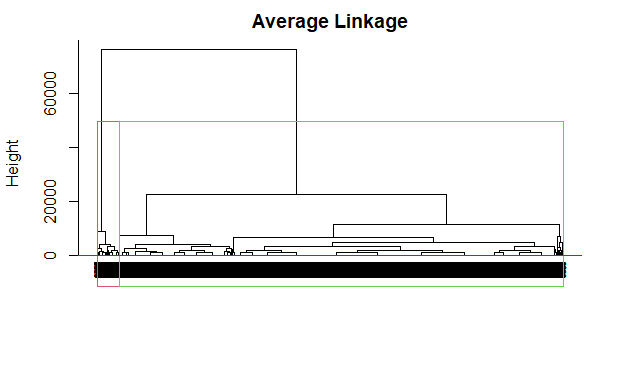
\includegraphics[width = \textwidth]{figure8.png}
	\caption{residual Vs Fitted}
	\label{Figure8}
\end{minipage}
\end{figure}


\subsection*{c.3 Evaluate the model performance}
we predict the output label based on two models. for comparing the accuracy we look at confusion matrix and count the correct classes. that shows accuracy of Logistic regression is a litter more. The total accuracy is around 82\%  which shows that there is more opportunity to improve the model performance.
one of reasons is that KNN works well with the numeric features, and in this dataset we have mix of both numeric and and categorical. 
Since logistic regression is a parametric model and 
Also in summary of model for statistical tests, we see that median of "Deviance Residuals" is 0.2600. In the coefficient part Pvalues of vehicle year and driving experience is quite small and shows both are statistically significant\cite{Gareth2013}. Also based on result of Vif() for our logistic regression it shows all variables are less than 10 that shows well independence between predictors, in table
\begin{table}[H]
	\centering
	 \caption{measure of multicollinearity}
	\begin{tabular}{rrrr}
		\hline
		& GVIF & Df & GVIF\verb|^|(1/(2*Df)) \\ 
		\hline
		age & 1.87 & 1.00 & 1.37 \\ 
		income & 1.63 & 3.00 & 1.08 \\ 
		driving\_experience & 2.48 & 1.00 & 1.58 \\ 
		annual\_mileage & 1.14 & 1.00 & 1.07 \\ 
		vehicle\_year & 1.09 & 1.00 & 1.04 \\ 
		vehicle\_type & 1.00 & 1.00 & 1.00 \\ 
		speeding\_violations & 1.84 & 1.00 & 1.36 \\ 
		past\_accidents & 1.49 & 1.00 & 1.22 \\ 
		\hline
	\end{tabular}
\end{table}




	\newpage
	\bibliographystyle{apa}
	\bibliography{Assignment2}
	
\end{document}